%/**
% * LaTeX thesis template (main file)
% * @author  : Alexander willner (willner@cs.uni-bonn.de)
% */

% /* include config ------------------------------------------------------ */
\newcommand{\metaFilename}{thesis_template}
\input{\metaFilename.config.tex}
%\excludecomment{finalComments}
\def\showDedication{1} % 1=show it, 0=hide it
% /* --------------------------------------------------------------------- */


% /* begin paper --------------------------------------------------------- */
\begin{document}
    \frontmatter
    \pagestyle{empty}
    \pagenumbering{alph}
    \begin{titlepage}
\rmfamily
\begin{flushleft}
%%\begin{center}
\LARGE{\textbf{\metaTitle}}\\
\normalsize

\vspace{1,4cm}
\textbf{\metaType}\\
\metaWhy\newline
\metaArticle~\metaFaculty\newline
\metaArticle~\metaUniversity\newline

\vspace{1,4cm}
\metaSubmitted\newline
\textbf{\metaAuthor}, \textbf{\metaDegree}\\
\metaBirthplace\newline

\vspace{1,4cm}
\metaCity, \metaDate\newline

\vspace{1,4cm}
Some \\
more \\
Text.\\

\vspace{1,4cm}
\hspace{-.4cm}
\begin{tabular}{ll}
First reviewer &: \metaFirstReviewerName\newline
Second reviewer &: \metaSecondReviewerName\newline
Day of submission &: \metaDateExam%
\end{tabular}
%%\end{center}
\end{flushleft}

\setlength{\wpYoffset}{40pt}
\ThisLROffsetCornerWallPaper{.2}{resources/images/logo}

\end{titlepage}

    \cleardoublepage
    %/**
% * LaTeX thesis template (deposition)
% * @author  : Alexander willner (willner@cs.uni-bonn.de)
% */

\vspace*{100mm}
\begin{minipage}{109.5mm}
\section*{Affidavit}
I hereby declare that the following thesis "\metaTitle" has been
written only by the undersigned and without any assistance from third
parties.\\

Furthermore, I confirm that no sources have been used in the preparation
of this thesis other than those indicated in the thesis itself.\\[2cm]
\metaCity, \metaDate
\end{minipage}

    \ifnum\showDedication > 0
    \cleardoublepage
      %/**
% * LaTeX thesis template (dedication)
% * @author  : Alexander willner (willner@cs.uni-bonn.de)
% */

\pdfbookmark{Dedication}{dedication}
\begin{center}
\Large{\metaDedication}
\end{center}

    \fi
    \cleardoublepage

    \pagestyle{headings}
    \pagenumbering{roman}
    \setcounter{page}{1}
    %/**
% * LaTeX thesis template (abstract)
% * @author  : Alexander willner (willner@cs.uni-bonn.de)
% */
\pdfbookmark{Abstract}{abstrct}
\chapter*{Abstract}\label{sec:abstract}
%\mtcaddchapter\addcontentsline{toc}{chapter}{Abstract}


\sidenote{Introduction and Problem Statement}
Suspendisse vel felis. Ut lorem lorem, interdum eu, tincidunt sit amet, laoreet vitae, arcu. Aenean faucibus pede eu ante. Praesent enim elit, rutrum at, molestie non, nonummy vel, nisl. Ut lectus eros, malesuada sit amet, fermentum eu, sodales cursus, magna. Donec eu purus. Quisque vehicula, urna sed ultricies auctor, pede lorem egestas dui, et convallis elit erat sed nulla. Donec luctus. Curabitur et nunc. Aliquam dolor odio, commodo pretium, ultricies non, pharetra in, velit. Integer arcu est, nonummy in, fermentum faucibus, egestas vel, odio.

\sidenote{Related Work and Research Questions}
\lipsum[6]

\sidenote{Research Contributions and how they've been validated}
This thesis contribution is severalfold. At first...
\lipsum[6]

\sidenote{Conclusions}
\lipsum[6]

%    \begin{quote}
%    "`\begin{CJK}{UTF8}{gbsn}不闻不若闻之,闻之不若见之,见之不若知之,知之不若行之;学至于行之而止矣。\end{CJK}"' -
%    \textit{Xunzi, Chinese philosopher (about 300-230 BC)}
%
%    "`not hearing is not as good as hearing, hearing is not as good as
%       seeing, seeing is not as good as mentally knowing, mentally knowing is
%       not as good as acting; true learning continues up to the point that
%       action comes forth [or, only when a thing produces action can it be said
%      to have been truly learned]"'
%    \end{quote}

\cleardoublepage
\chapter*{Zusammenfassung}\label{sec:zusammenfassung}
\sidenote{Einleitung und Problemstellung}
\lipsum[6]

\sidenote{Verwandte Arbeiten und Forschungsfragen}
\lipsum[6]

\sidenote{Wissenschaftlicher Beitrag}
\lipsum[6]

\sidenote{Zusammenfassung}
\lipsum[6]
\cleardoublepage

    \ifnum\showDedication > 0
    %/**
% * LaTeX thesis template (ackknowledgment)
% * @author  : Alexander willner (willner@cs.uni-bonn.de)
% */

\chapter*{Acknowledgments}
This template was conducted during my time as ...

First and foremost, I would like to thank ...

I would like to express special thanks to ...

\vspace{0.5in}
\begin{flushright}
  \metaCity, \metaDate
\end{flushright}

    \fi
    \cleardoublepage

    \phantomsection
    %/**
% * LaTeX thesis template (tables)
% * @author  : Alexander willner (willner@cs.uni-bonn.de)
% */

\pdfbookmark{Table of Contents}{toc}
\tableofcontents
%\mtcaddchapter\addcontentsline{toc}{chapter}{Table of Contents}
\cleardoublepage

\listoffigures
\mtcaddchapter\addcontentsline{toc}{chapter}{\listfigurename}
\cleardoublepage

\listoftables
\mtcaddchapter\addcontentsline{toc}{chapter}{\listtablename}
\cleardoublepage

\lstlistoflistings
\mtcaddchapter\addcontentsline{toc}{chapter}{List of Algorithms}
\cleardoublepage

\chapter*{List of Abbreviations and Symbols}
\mtcaddchapter\addcontentsline{toc}{chapter}{List of Abbreviations and Symbols}

\cleardoublepage

    \cleardoublepage

    \mainmatter
    \pagenumbering{arabic}
    \setcounter{page}{1}
    \linenumbers
    %/**
% * LaTeX thesis template (introduction)
% * @author  : Alexander willner (willner@cs.uni-bonn.de)
% */

\cleardoublepage\chapter{Introduction}\minitoc\label{sec:introduction}\vspace{.5cm}
\note{general introduction to the context and the core of the thesis}
\noindent\lipsum[7]

\section{Problem Statement and Research Questions}
\lipsum[7]

\section{Reasearch Contributions}
\lipsum[7]
\begin{itemize}
  \item[\textbf{Goal 1}:]
  \lipsum[5]

  \item[\textbf{Goal 2}:]
  \lipsum[5]

  \item[\textbf{Goal 3}:]
  \lipsum[5]

  \item[\textbf{Goal 4}:]
  \lipsum[5]
\end{itemize}

\section{Outline of the Thesis}
We conclude with an outline of the thesis and a short summary of each chapter.
\begin{itemize}
  \item[\textbf{\chaptername~\ref{sec:relatedwork}}:]
  \note{related work}
  \lipsum[5]

  \item[\textbf{\chaptername~\ref{sec:assumptions}}:]
  \note{assumptions}
  \lipsum[5]

  \item[\textbf{\chaptername~\ref{sec:concept}}:]
  \note{concept}
  \lipsum[5]

  \item[\textbf{\chaptername~\ref{sec:evaluation}}:]
  \note{evaluation}
  \lipsum[5]

  \item[\textbf{\chaptername~\ref{sec:summary}}:]
  \note{summary}
  \lipsum[5]
\end{itemize}


    %/**
% * LaTeX thesis template (related work)
% * @author  : Alexander willner (willner@cs.uni-bonn.de)
% */

\cleardoublepage\chapter{Related Work and Research Gaps}\minitoc\label{sec:relatedwork}\vspace{.5cm}
\sidenote{review of relevant work on different sub problems.}
\noindent\lipsum[7]

\section{Summary}
\lipsum[5]

    %/**
% * LaTeX thesis template (assumptions)
% * @author  : Alexander willner (willner@cs.uni-bonn.de)
% */

\cleardoublepage\chapter{Assumptions, Objectives and Scope}\minitoc\label{sec:assumptions}\vspace{.5cm}
\sidenote{text}
\noindent\lipsum[7]

\section{Use Cases and Assumptions}
\lipsum[5]

\section{Requirements and Objectives}
\lipsum[5]

\section{Test}

\cite{Waitzman:1999}

\small
\begin{equation}
  \begin{array}{l}
    \displaystyle t^{p_d}_{fw}(d) = max_{d}(t_{child_{i}}) \\
    \displaystyle t^{p_d}_{db}(d) = \sum_{i=1}^{d} t_{db_{i}} \\
    \displaystyle t^{p_d}_{pc}(n,d) =
    	\begin{cases}
        	t_{pc}(d) + c(n) & \text{if $d = 1$,}\\
        	t_{pc}(d) + c(n) + max(t_{avail}(d)) & \text{if $d>1$.}\\
        \end{cases}
  \end{array}
  \label{eq:var_idb}
\end{equation}
\normalsize

\begin{figure}
    \centering
    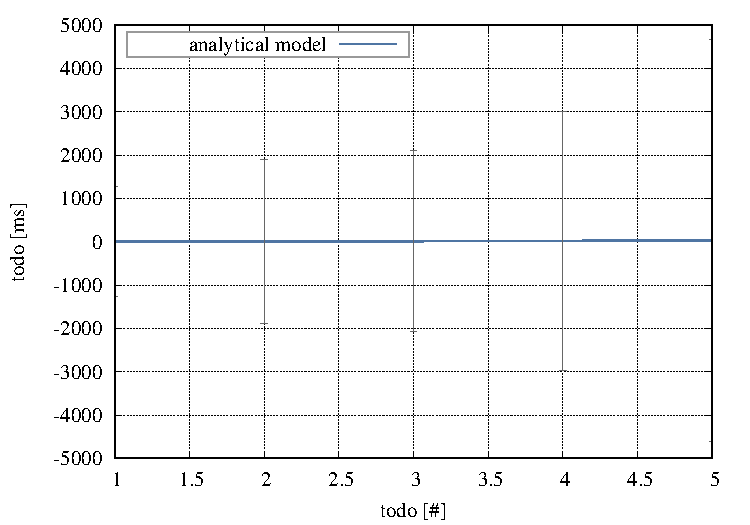
\includegraphics[width=.65\textwidth]{resources/images/example1.pdf}
    \caption{Example image.}
    \label{fig:example1}
\end{figure}

\begin{figure}
    \begin{subfigure}[b]{.5\textwidth}
      \centering
      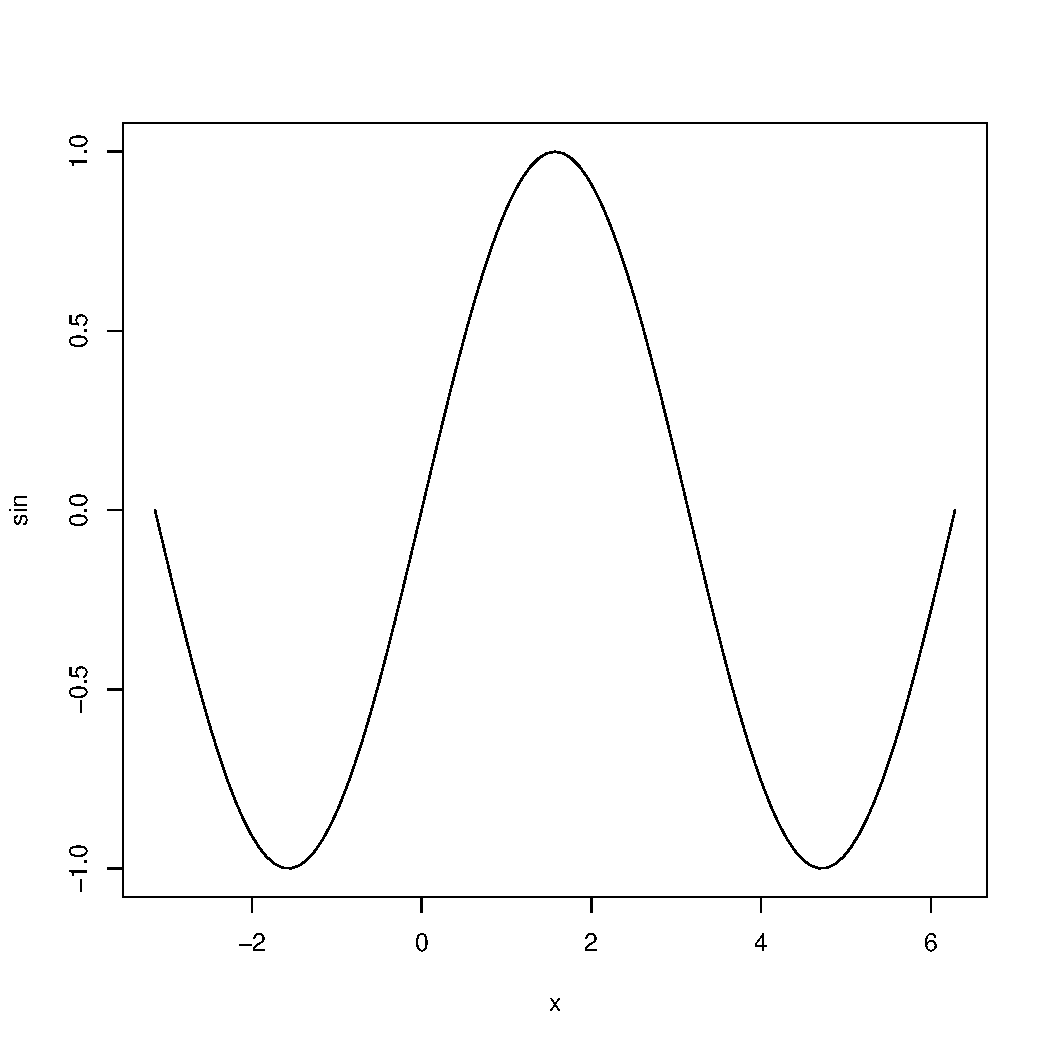
\includegraphics[width=.95\textwidth,frame]{resources/images/example2}
      \caption{example2}\label{fig:example2}
    \end{subfigure}~\begin{subfigure}[b]{.5\textwidth}
      \centering
      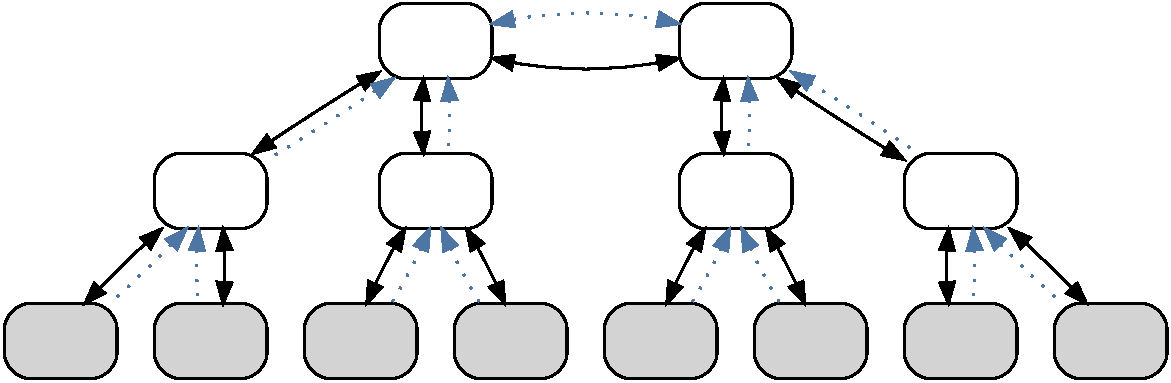
\includegraphics[width=.95\textwidth,frame]{resources/images/example3}
      \caption{example3}\label{fig:example3}
    \end{subfigure}
    \caption{Example images}\label{fig:exammple2_3}
\end{figure}

\begin{center}
  \begin{tabularx}{\textwidth}{ll}
      \caption{Example table}\label{tbl:exampletable}\\
        \toprule\textbf{Name} & \textbf{Age}\\\midrule
        \endfirsthead
        \toprule\textbf{Name} & \textbf{Age}\\\midrule
        \endhead
        \midrule
            \multicolumn{2}{r}{\emph{Continued on next page}}
        \endfoot
        \bottomrule
        \endlastfoot
       Hans           & 80             \\
       Heinrich       & 77             \\
       Herbert        & 84             \\
    \end{tabularx}
\end{center}

\lstset{language=Java, caption=Example Code., %
label=lst:example, numbers=left, stepnumber=1}
\lstinputlisting{resources/code/example.java}

\section{Summary}
\lipsum[5]

    %/**
% * LaTeX thesis template (anaysis)
% * @author  : Alexander willner (willner@cs.uni-bonn.de)
% */

\cleardoublepage\chapter{Reseach Question 1}\minitoc\label{sec:concept}\vspace{.5cm}
\note{Introduction and Problem Statement. Up to 40 pages.}
\noindent\lipsum[7]
\section{Related Work}
\note{some text}
\label{sec:concept:relatedwork}
\lipsum[7]
\section{Own Approach / Concept / Contribution}
\note{some text}
\label{sec:concept:approach}
\lipsum[7]
\section{Evaluation}
\note{some text}
\label{sec:concept:evaluation}
\lipsum[7]

\section{Discussion}
\note{some text}
\label{sec:concept:discussion}
\lipsum[7]
\section{Chapter Summary}
\note{some text}
\label{sec:concept:summary}
\lipsum[7]

    %/**
% * LaTeX thesis template (evaluation)
% * @author  : Alexander willner (willner@cs.uni-bonn.de)
% */

\cleardoublepage\chapter{Performance Evaluation}\minitoc\label{sec:evaluation}\vspace{.5cm}
\sidenote{simulation environment, metrics, parameter}
\noindent\lipsum[7]

\section{General Model}\label{sec:model}
\lipsum[5]

\section{Considered Metrics}\label{sec:metrics}
\lipsum[5]

\section{Analytical Evaluation}\label{sec:analytic}
\lipsum[5]

\section{Simluative Evaluation}\label{sec:sim}
\lipsum[5]

\section{Chapter Summary}\label{sec:result}
\sidenote{Lessons learned and transferability}
\lipsum[5]


    %/**
% * LaTeX thesis template (summary)
% * @author  : Alexander willner (willner@cs.uni-bonn.de)
% */

\cleardoublepage\chapter{Conclusions, Discussions and Future Work}\minitoc\label{sec:summary}\vspace{.5cm}
\sidenote{Reference to problem, listing from inferences, sorted from important to unimportant. About 2--4 pages. We're now on page 140.}
\noindent\lipsum[7]

\section{Results}
\sidenote{Listing of the scientific contributions and what is new}
\label{sec:summary:results}
\lipsum[7]

\section{Deployability}
\sidenote{On how the results can be used}
\label{sec:summary:deployability}
\lipsum[7]

\section{Future Work}
\sidenote{Open research questions}
\label{sec:summary:futurework}
\lipsum[7]


    \nolinenumbers
    \cleardoublepage

    \appendix
    \pagenumbering{Roman}
    \setcounter{page}{1}
    %/**
% * LaTeX thesis template (appendix)
% * @author  : Alexander willner (willner@cs.uni-bonn.de)
% */


\cleardoublepage\chapter{Formal Description of Something}\minitoc\label{sec:formal}\vspace{.5cm}
\note{Some appendix.}
\noindent\lipsum[7]

\cleardoublepage\chapter{Some more Evaluation Results}\minitoc\label{sec:moreeval}\vspace{.5cm}
\note{Some appendix.}
\noindent\lipsum[7]

    %/**
% * LaTeX thesis template (unsorted)
% * @author  : Alexander willner (willner@cs.uni-bonn.de)
% */

\cleardoublepage\chapter{\LaTeX~Tests}\minitoc\label{sec:latextest}\vspace{.5cm}
\sidenote{Some unsorted \LaTeX~tests}
\noindent\lipsum[7]

\begin{itemize}
  \item[\textbf{Acronyms}:] \ac{SONA} again \ac{SONA}. And \acp{SLA} also \ac{SLA} again \acp{SLA}. And \acf{SLA}.
  \item[\textbf{Index}:] Index\index{Index} and Subindex\index{Index!Subindex} in the \appendixname.
  \item[\textbf{Mote annotations}:] \ac{H2O}.
\end{itemize}




    \cleardoublepage
    %\bibliographystyle{abbrv}
    %% To list uncited references (disable the line above):
    \bibliographystyle{unsrt}
    \cite{uncited}
    \nocite{*}

    \bibliography{\metaFilename,build}
    \mtcaddchapter\addcontentsline{toc}{chapter}{Bibliography}

    \backmatter
    \cleardoublepage
    \renewcommand{\indexname}{Index}
    \printindex
\end{document}
% /* ----------------------------------------------------------- end paper */
